% Created 2020-05-22 Fri 14:39
% Intended LaTeX compiler: pdflatex
\documentclass[presentation]{beamer}
\usepackage[utf8]{inputenc}
\usepackage[T1]{fontenc}
\usepackage{graphicx}
\usepackage{grffile}
\usepackage{longtable}
\usepackage{wrapfig}
\usepackage{rotating}
\usepackage[normalem]{ulem}
\usepackage{amsmath}
\usepackage{textcomp}
\usepackage{amssymb}
\usepackage{capt-of}
\usepackage{hyperref}
\usetheme{UoB}
\author{Mark Blyth}
\date{\textit{[2020-05-25 Mon]}}
\title{Systematic testing of GPR kernels}
\hypersetup{
 pdfauthor={Mark Blyth},
 pdftitle={Systematic testing of GPR kernels},
 pdfkeywords={},
 pdfsubject={},
 pdfcreator={Emacs 26.3 (Org mode 9.1.9)}, 
 pdflang={English}}
\begin{document}

\maketitle

\section{Background}
\label{sec:org57afbde}
\begin{frame}[label={sec:org416965d}]{Week's goals}
\begin{itemize}
\item Redraft paper 
\begin{itemize}
\item \emph{[done]}
\end{itemize}
\item Teaching stuff 
\begin{itemize}
\item \emph{[done]}
\end{itemize}
\item Do some more systematic testing of the GPR kernels
\begin{itemize}
\item \emph{[in progress]}
\end{itemize}
\end{itemize}
\end{frame}

\section{Noise pics}
\label{sec:org27dcaf9}
\begin{frame}[label={sec:org61bd94c}]{Kernel fitting}
\begin{itemize}
\item Tried the kernels I coded, on several models
\item Tried with and without noise
\item Found some interesting results\ldots{}
\end{itemize}
\end{frame}

\begin{frame}[label={sec:org0665012}]{Good LL, bad fit}
\begin{center}
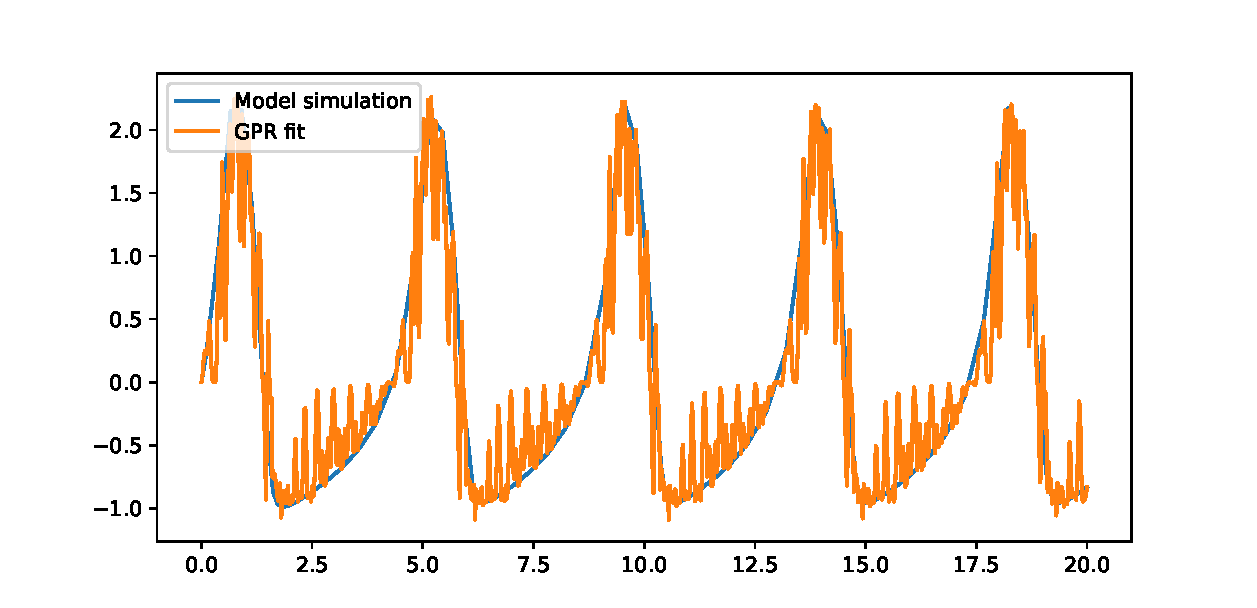
\includegraphics[width=.9\textwidth]{./HRFast_standard.pdf}
\end{center}

Log-likelihood = -132  \hfill \(\sigma_n^2=0\) \hfill periodic kernel, HRFast model
\end{frame}

\begin{frame}[label={sec:org94b4652}]{Good LL, good fit}
\begin{center}
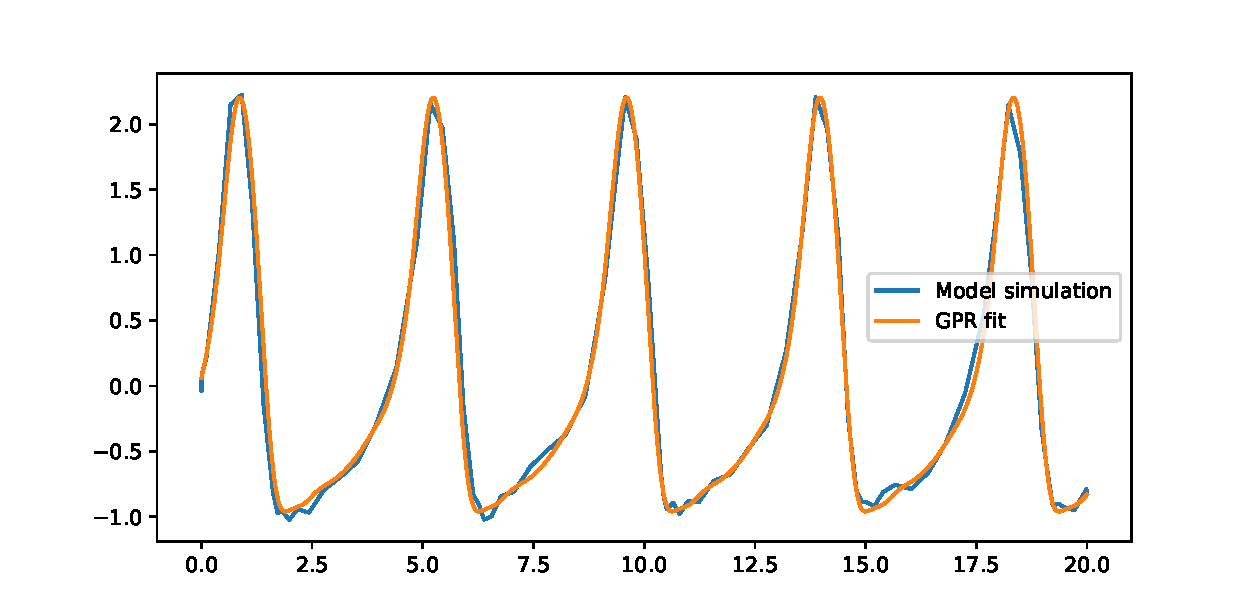
\includegraphics[width=.9\textwidth]{./HRFast_n_n.pdf}
\end{center}

Log-likelihood = -100\hfill \(\sigma_n^2=0.05\)\hfill periodic kernel, HRFast model
\end{frame}

\begin{frame}[label={sec:orgb1a475c}]{Bad LL, good fit}
\begin{center}
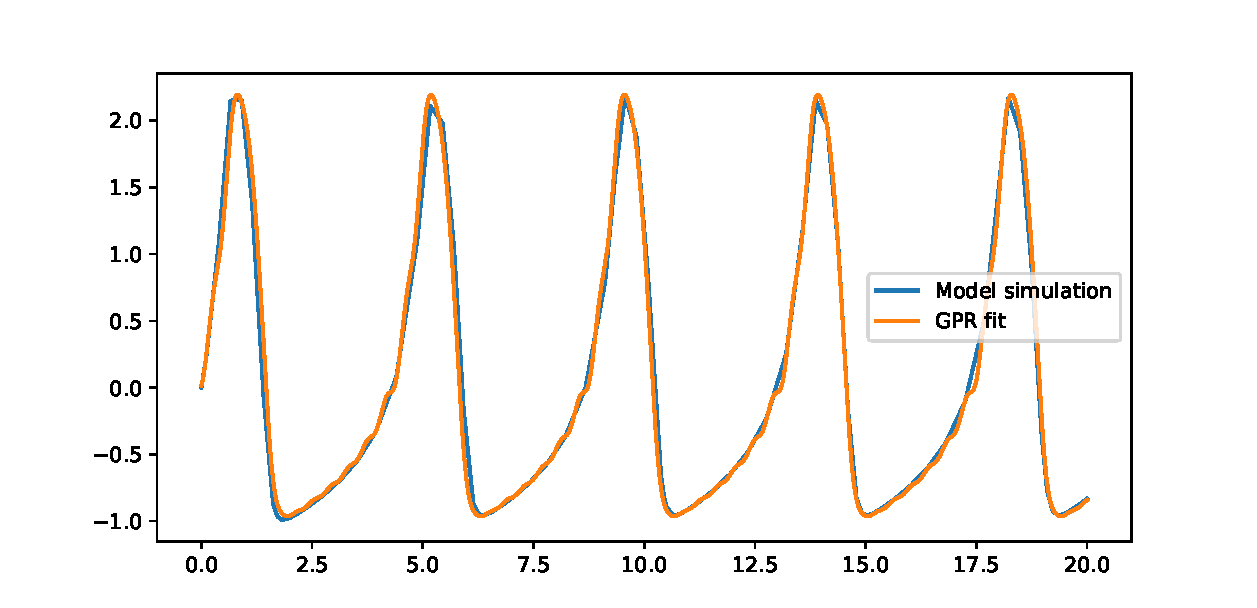
\includegraphics[width=.9\textwidth]{./HRFast_noise_clean.pdf}
\end{center}

Log-likelihood = -377,038\hfill \(\sigma_n^2 = 0\)\hfill periodic kernel, HRFast model
\end{frame}

\begin{frame}[label={sec:org958b550}]{How good is good enough?}
\begin{center}
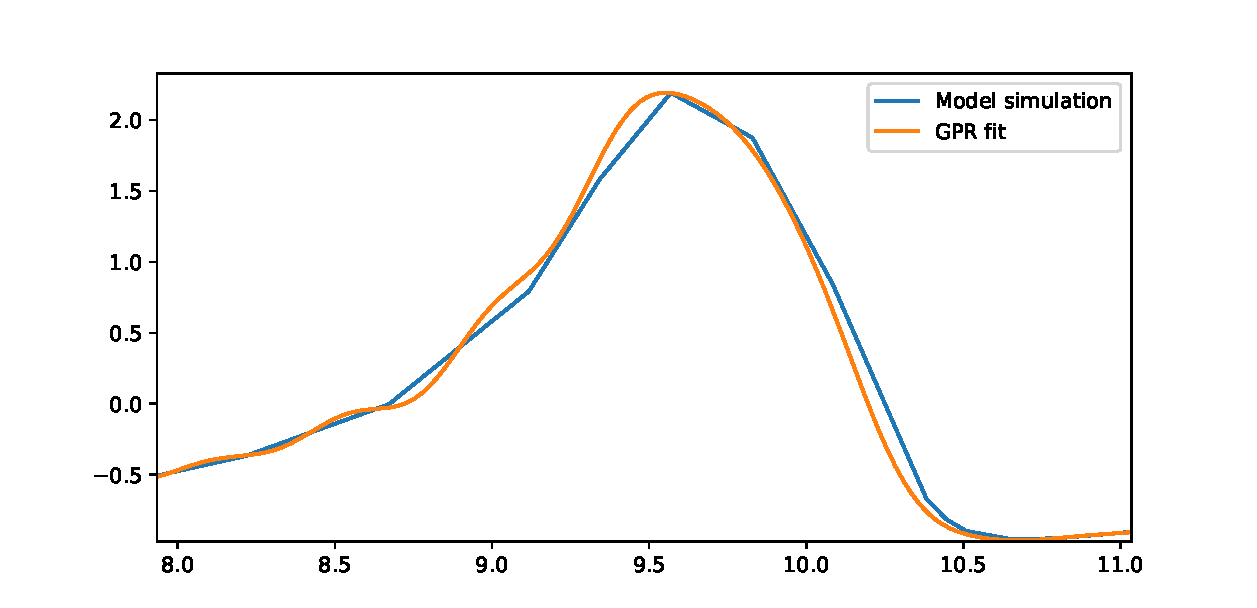
\includegraphics[width=.9\textwidth]{./wiggles.pdf}
\end{center}

Even the best-achievable fit isn't perfect; gets worse with more data
\end{frame}

\section{Tables}
\label{sec:orgbe9f612}
\begin{frame}[label={sec:org21020c1}]{Log-likelihoods}
\begin{center}
\begin{tabular}{lrrrr}
\hline
 & My SEKernel & Modulo kernel & Periodic kernel & \(\sigma_n^2\)\\
\hline
FitzhughNagumo & -289 & -283 & -290 & 0.1\\
HR fast & -277 & -287 & -284 & 0.05\\
Hodgkin Huxley & -6170 & -2690 & -2657 & 2\\
\hline
\end{tabular}
\end{center}

\vfill

\begin{center}
\begin{tabular}{lrrr}
\hline
 & My SEKernel & Modulo kernel & Periodic kernel\\
\hline
FitzhughNagumo & -135 & -178 & -170\\
HR fast & -114 & -152 & -132\\
Hodgkin Huxley & -8547 & -9952 & -9878\\
\hline
\end{tabular}
\end{center}

Good LL, bad fits
\end{frame}

\begin{frame}[label={sec:org4f8845e}]{Log-likelihoods}
\begin{center}
\begin{tabular}{llll}
\hline
 & My SEKernel & Modulo kernel & Periodic kernel\\
\hline
FitzhughNagumo & -135 & -457,451 & -456,778\\
HR fast & -1,120,469 & -145,659 & -377,038\\
Hodgkin Huxley & -175,468,920 & -39,092,086 & -39,117,518\\
\hline
\end{tabular}
\end{center}

\vfill

Good fits, bad LL
\end{frame}


\section{Discussion}
\label{sec:org5e023fd}
\begin{frame}[label={sec:orgf3ffdc8}]{Log-likelihoods}
\begin{itemize}
\item LL is meant to prevent overfitting, but it doesn't
\item Can have a terrible fit and a good LL
\item Can have a terrible LL and a good fit
\item LL is not always a good measure of success
\end{itemize}
\end{frame}

\begin{frame}[label={sec:org739cda7}]{Causes of weirdness}
\begin{itemize}
\item No noise means small deviations give large LL penalties
\begin{itemize}
\item Noise-free models are fitted with \(\sigma_n^2 = 0\)
\item Overfitting happens: model tries too hard to match provided datapoints
\item Loses ability to generalise (becomes dippy)
\vfill
\end{itemize}
\item Noisy fits help
\begin{itemize}
\item No exact datapoints, so model is forced to average out noise
\item Reduces the maximum goodness-of-fit, and forces the model to more cleverly estimate posterior
\item Less overfitting, so more generalisable, reducing dipping
\end{itemize}
\end{itemize}
\end{frame}

\begin{frame}[label={sec:org869c79d}]{Jitter}
Overfitting can sometimes be cured by adding some noise


\vfill

\begin{itemize}
\item Jitter is manaully added noise
\item Adding jitter has the potential to offset overfitting, by pretending there's noise when there isn't
\item Can give a more sensible LL value
\begin{itemize}
\item LL depends on the size of the jitter, impossible to choose a `right' value \emph{[not strictly true]}
\end{itemize}
\end{itemize}

\vfill

Adding jitter isn't a useful method, as it degenerates into regular noisy data-fitting.
\end{frame}


\begin{frame}[label={sec:orgac78912}]{Best approach}
\begin{itemize}
\item Add noise into data
\item Fit other hyperparameters, with signal noise fixed at whatever noise variance we added in
\begin{itemize}
\item Maximise log-likelihood
\end{itemize}
\item Reuse these results on the noise-free case
\item We can do this, as the fitted hyperparameters will take the same value, independent of clean or noisy signals

\vfill
\end{itemize}

Fitting to noisy data gives the best possible results, regardless of what the LL says
\begin{itemize}
\item It's still not always a good enough fit\ldots{}
\end{itemize}
\end{frame}

\section{HH results}
\label{sec:orgdaf383b}
\begin{frame}[label={sec:orgd32516e}]{Nonstationarity}
\begin{center}
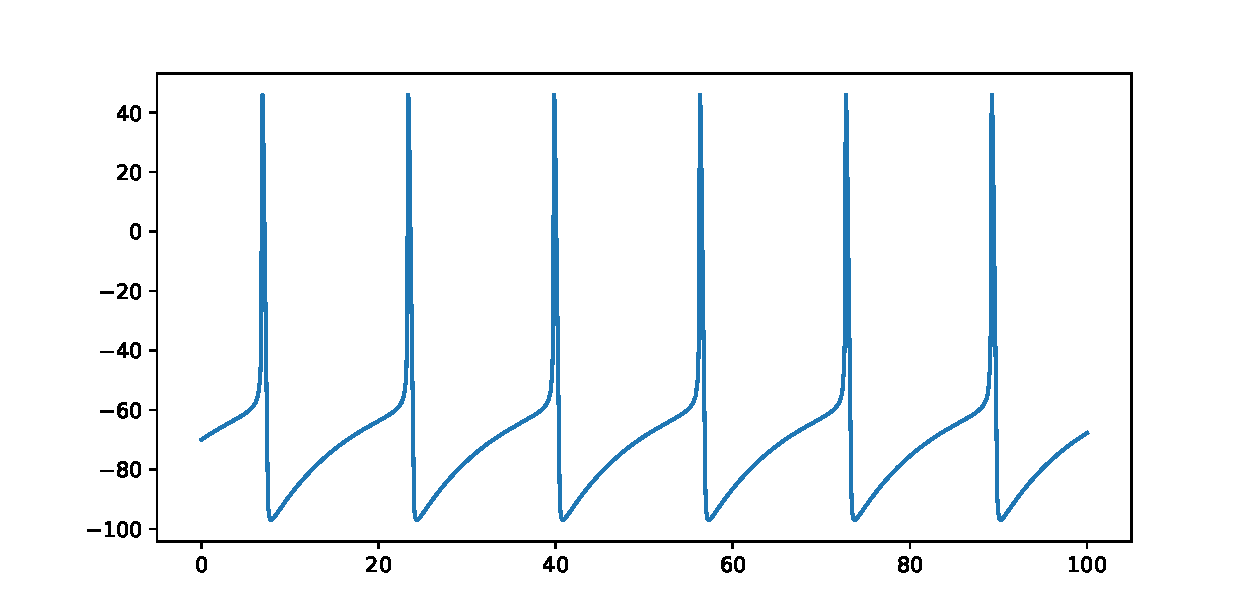
\includegraphics[width=.9\textwidth]{./HHraw.pdf}
\end{center}

Hodgkin-Huxley is a good test of the models -- nonstationary, and realistic
\end{frame}

\begin{frame}[label={sec:org462fc9f}]{Nonstationarity}
\begin{center}
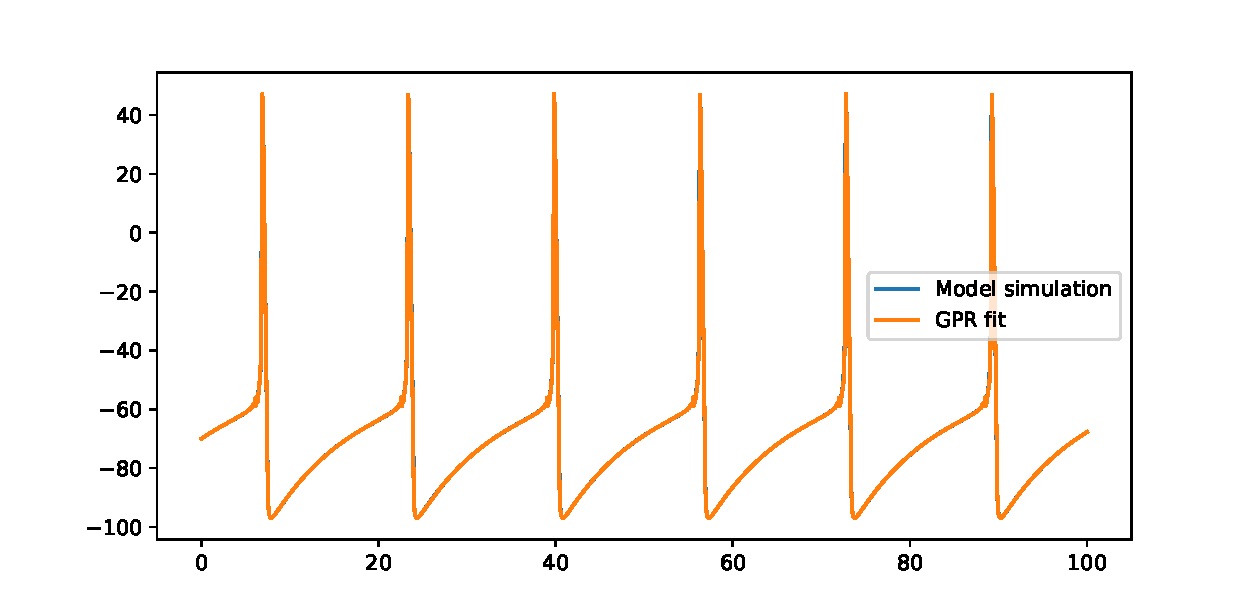
\includegraphics[width=.9\textwidth]{./HH_good.pdf}
\end{center}

Looks good, right? \hfill Fitted on \(\sigma_n^2=2\) \hfill Tested on \(\sigma_n^2 = 0\)
\end{frame}

\begin{frame}[label={sec:orgd52c057}]{Nonstationarity}
\begin{center}
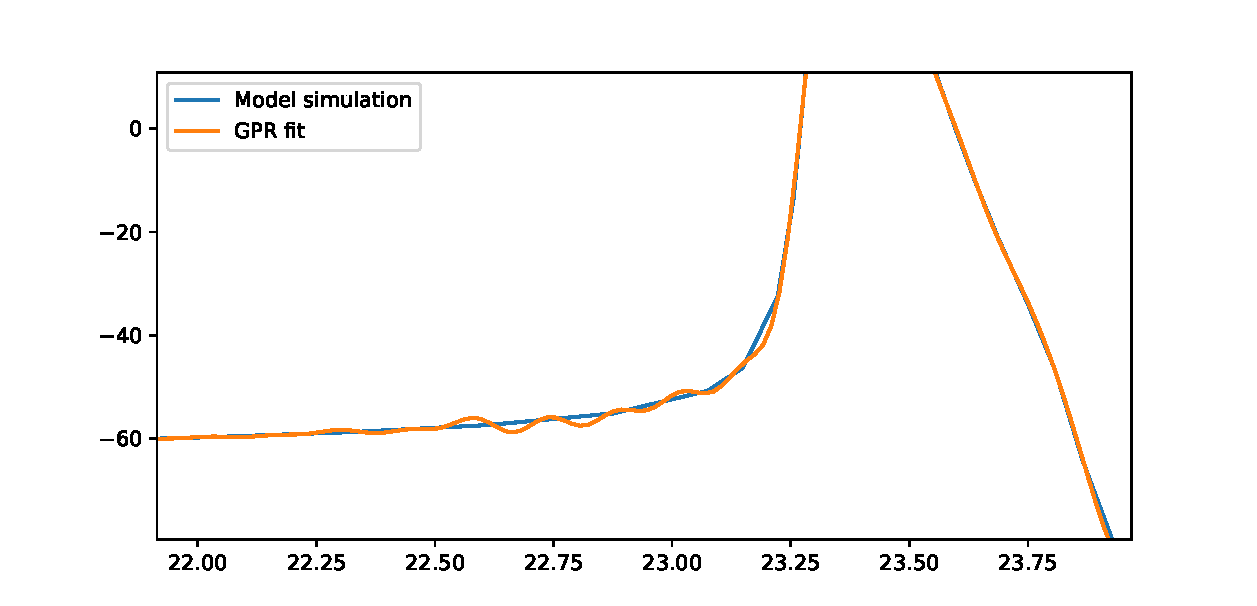
\includegraphics[width=.9\textwidth]{./HH_good_2.pdf}
\end{center}

Still looks good \hfill Fitted on \(\sigma_n^2=2\) \hfill Tested on \(\sigma_n^2 = 0\)
\end{frame}

\begin{frame}[label={sec:org50016a8}]{Nonstationarity}
\begin{center}
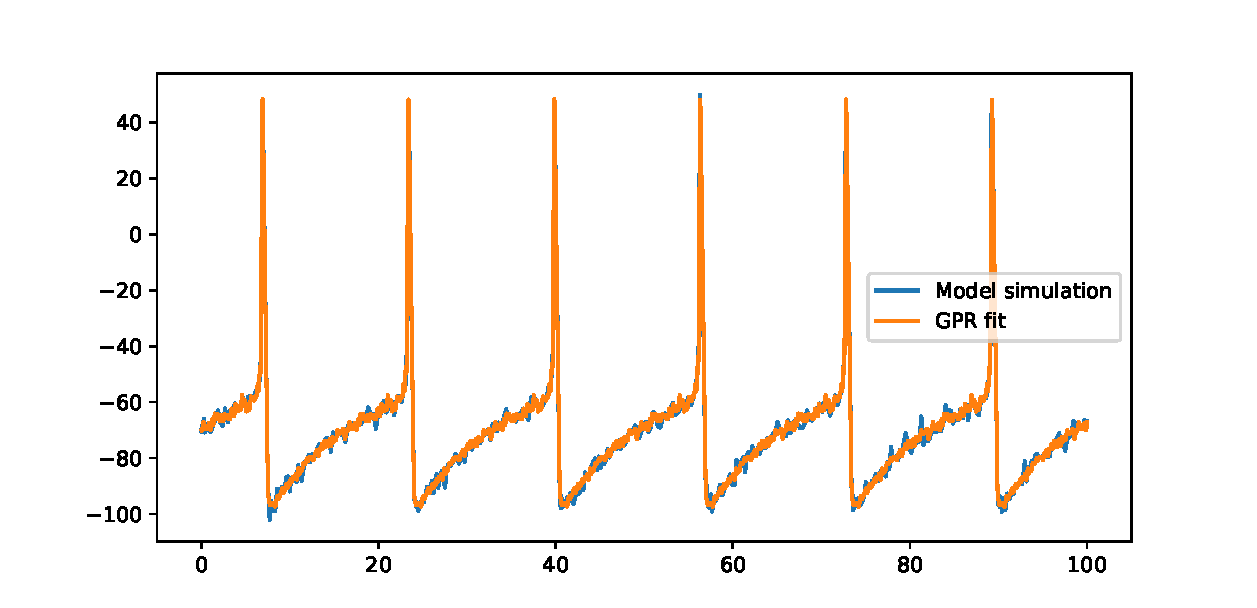
\includegraphics[width=.9\textwidth]{./HH_bad.pdf}
\end{center}

Uh oh\ldots{} \hfill Fitted on \(\sigma_n^2=2\) \hfill Tested on \(\sigma_n^2 = 2\)
\end{frame}

\begin{frame}[label={sec:org43d7b8d}]{Nonstationarity}
\begin{center}
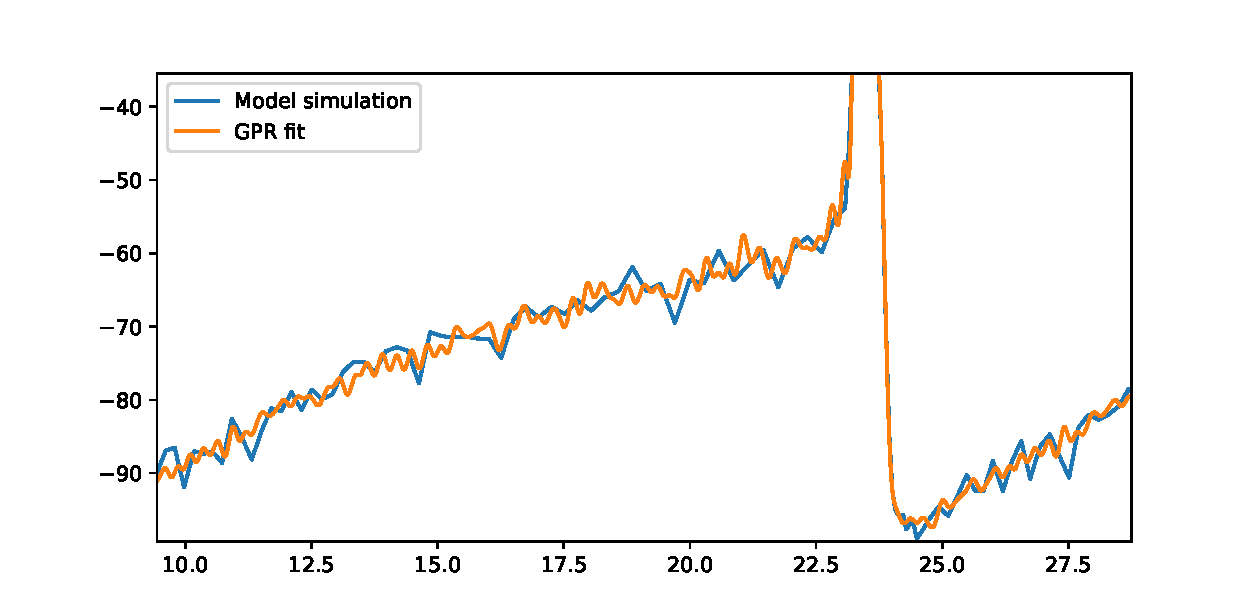
\includegraphics[width=.9\textwidth]{./HH_bad_2.pdf}
\end{center}

Uh oh\ldots{} \hfill Fitted on \(\sigma_n^2=2\) \hfill Tested on \(\sigma_n^2 = 2\)
\end{frame}

\begin{frame}[label={sec:org4b820eb}]{Nonstationarity}
Hodgkin-Huxley fit loses the ability to average out noise
    \vfill
\begin{itemize}
\item Requires very small lengthscales to model spikes
\item Small lengthscales overfit the noise
\item We end up with \emph{more} noise in the model than in the original signal!
\begin{itemize}
\item Worse results by fitting a model
\end{itemize}
\end{itemize}
\vfill
Nonstationarity would fix this!
\end{frame}

\section{Next steps}
\label{sec:orgcb0aeb7}
\begin{frame}[label={sec:org1b145a0}]{Next steps: part 1}
Other GPR methods:
\begin{itemize}
\item Function-space distribution over kernels
\item Generalised spectral mixture kernels
\item Switching kernel

\vfill
\end{itemize}

Implement and test these on the shown datasets
\end{frame}

\begin{frame}[label={sec:org3fbfd7d}]{Next steps: part 2}
Lit-review of some other techniques I've spotted \emph{[useful for a paper]}

\vfill

Implement and test some other methods:
\begin{itemize}
\item GOAL: black-box data model \emph{[parametric or non-parametric]}
\item NARMAX \emph{[simple nonlinear timeseries models]}
\begin{itemize}
\item Popular in systems identification community
\end{itemize}
\item Neural ODEs \emph{[often combines NNs with GPs for latent ODE models]}
\item Bayesian free-knot splines
\begin{itemize}
\item Powerful for scalar signals!
\end{itemize}
\end{itemize}
\end{frame}
\end{document}
